\chapter{METODOLOGI}

% Ubah konten-konten berikut sesuai dengan isi dari metodologi

\section{Desain Rangkaian PWM AC \emph{Chopper}}
\label{sec:desain-pwm-ac-chopper}

Bagian ini membahas proses perancangan rangkaian daya dan sistem kontrol
PWM AC \emph{chopper} yang digunakan untuk mengatur tegangan suplai motor
pompa air satu fasa. Perancangan meliputi pemilihan topologi, penentuan
komponen saklar daya (IGBT), perhitungan rangkaian \emph{snubber}, dan
penentuan \emph{dead time} untuk mencegah \emph{shoot-through}. Skema
keseluruhan sistem yang dirancang ditunjukkan pada
Gambar~\ref{fig:skema-sistem-alat}.

\begin{figure} [H] \centering
  % Nama dari file gambar yang diinputkan
  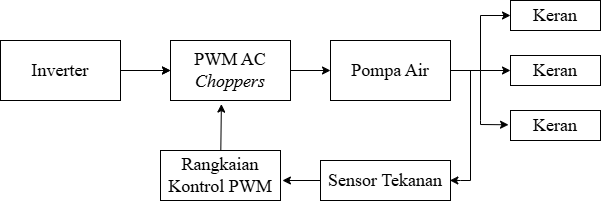
\includegraphics[scale=0.55]{gambar/skema_alat_rev.png}
  % Keterangan gambar yang diinputkan
  \caption{Skema Sistem Alat}
  % Label referensi dari gambar yang diinputkan
  \label{fig:skema-sistem-alat}
\end{figure}

Pada sistem ini, sensor tekanan air memberikan umpan balik tekanan aktual
ke mikrokontroler STM32. STM32 membandingkan nilai tekanan tersebut
dengan \emph{setpoint} dan menghasilkan sinyal kendali berbasis
\emph{neural network} berupa \emph{duty cycle} PWM. Sinyal PWM tersebut
diteruskan ke rangkaian \emph{gate driver} untuk menggerakkan IGBT pada
rangkaian PWM AC \emph{chopper} sehingga tegangan input ke motor pompa
dapat diatur sesuai kebutuhan.

\subsection{Penentuan Topologi dan IGBT}
\label{sec:penentuan-topologi-dan-igbt}

Rangkaian PWM AC \emph{chopper} dirancang menggunakan topologi
\emph{full-bridge} empat IGBT yang ditunjukkan pada
Gambar~\ref{fig:skematik-pwm-ac-chopper}. Topologi ini memungkinkan
pemotongan (\emph{chopping}) tegangan AC secara \emph{bipolar} sehingga
didapatkan bentuk gelombang tegangan keluaran yang simetris pada kedua
sisi siklus. IGBT dipicu oleh pasangan sinyal PWM komplementer
(keempat IGBT bekerja sebagai dua pasang kaki \emph{leg}).

\begin{figure} [H] \centering
  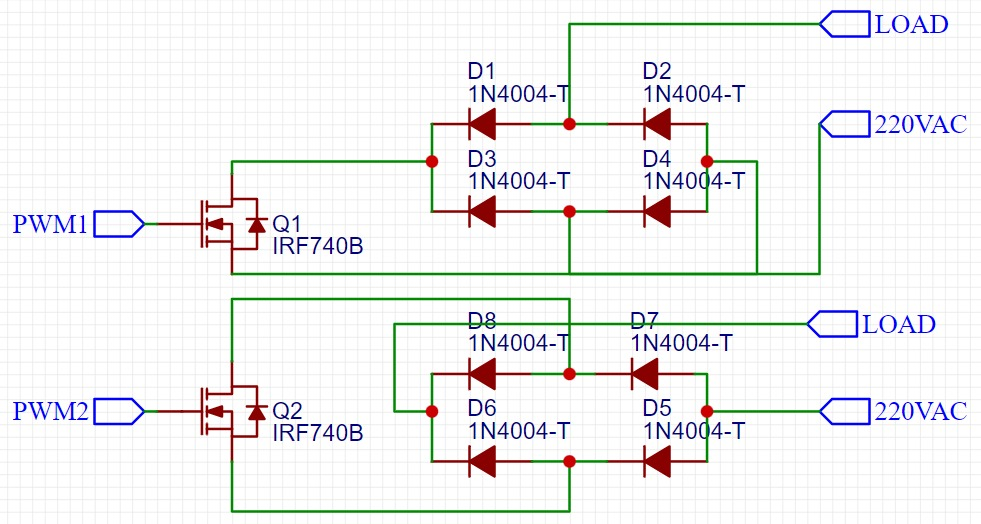
\includegraphics[scale=0.35]{gambar/RANGKAIAN.jpg}
  \caption{Skematik PWM AC \emph{Chopper}}
  \label{fig:skematik-pwm-ac-chopper}
\end{figure}

Pemilihan IGBT dilakukan dengan mempertimbangkan parameter berikut.
\begin{enumerate}
  \item Tegangan \emph{collector--emitter} maksimum ($V_{CES}$) yang
        lebih tinggi dari tegangan puncak input AC dengan faktor
        keamanan.
  \item Arus kolektor kontinu ($I_C$) yang mampu melewatkan arus beban
        pompa pada kondisi terberat.
  \item Tegangan saturasi (\emph{on-state}) $V_{CE(sat)}$ yang rendah
        untuk menekan rugi konduksi dan pemanasan.
  \item Kecepatan \emph{switching} (waktu tunda \emph{turn-on} dan
        \emph{turn-off}) yang singkat pada frekuensi PWM yang
        direncanakan.
  \item Ketersediaan di pasaran lokal dan referensi desain.
\end{enumerate}

Dengan pertimbangan di atas, pada penelitian ini digunakan IGBT
\textbf{FGH40N120AN} produksi ON Semiconductor dengan teknologi
NPT (Non-Punch Through). Spesifikasi penting IGBT yang digunakan
ditunjukkan pada Tabel~\ref{tab:spesifikasi-igbt}.

\begin{table}[H]
  \centering
  \caption{Spesifikasi Penting IGBT FGH40N120AN}
  \label{tab:spesifikasi-igbt}
  \begin{tabularx}{\linewidth}{|c|>{\raggedright\arraybackslash}X|c|c|c|}
  \hline
  \textbf{Parameter} & \textbf{Simbol} & \textbf{Min} & \textbf{Tip.} & \textbf{Maks.} \\
  \hline
  Tegangan \emph{collector--emitter} & $V_{CES}$ & 1200 V & --- & --- \\
  \hline
  Arus kolektor @ $T_C = 100^{\circ}$C & $I_C$ & --- & --- & 40 A \\
  \hline
  Tegangan saturasi @ $I_C = 40$ A & $V_{CE(sat)}$ & --- & 2,6 V & 3,2 V \\
  \hline
  Tegangan ambang \emph{gate--emitter} & $V_{GE(th)}$ & 3,5 V & 5,5 V & 7,5 V \\
  \hline
  \emph{Turn-on} delay, $T_C = 25^{\circ}$C & $t_{d(on)}$ & --- & 15 ns & --- \\
  \hline
  \emph{Turn-off} delay, $T_C = 25^{\circ}$C & $t_{d(off)}$ & --- & 110 ns & --- \\
  \hline
  \emph{Turn-on} delay, $T_C = 125^{\circ}$C & $t_{d(on)}$ & --- & 20 ns & --- \\
  \hline
  \emph{Turn-off} delay, $T_C = 125^{\circ}$C & $t_{d(off)}$ & --- & 120 ns & --- \\
  \hline
  Waktu \emph{rise} & $t_r$ & --- & 20 ns & --- \\
  \hline
  Waktu \emph{fall} & $t_f$ & --- & 40 ns & 80 ns \\
  \hline
  Total gate charge & $Q_g$ & --- & 220 nC & --- \\
  \hline
  \end{tabularx}
\end{table}

Pada Tabel~\ref{tab:spesifikasi-igbt} terlihat bahwa
$V_{CES} = 1200$ V jauh melebihi tegangan puncak AC 220~V
($\hat{V} = 311$ V), sehingga perangkat ini memiliki margin
tegangan yang lebih dari cukup untuk aplikasi AC \emph{chopper}
1 fasa. Kapasitas arus kolektor 40~A pada $T_C = 100^{\circ}$C
juga lebih dari cukup untuk melayani pompa air GP125 125~W
(arus nominal $<$ 1~A pada 220~V). Penempatan \emph{heatsink}
dilakukan untuk menjaga suhu kerja IGBT agar tetap berada di
bawah batas maksimum $150^{\circ}$C yang diizinkan pada
datasheet.

\subsection{Penentuan Rangkaian \emph{Snubber}}
\label{sec:penentuan-snubber}

Rangkaian \emph{snubber} digunakan pada bagian saklar daya PWM AC
\emph{chopper} untuk meredam lonjakan tegangan dan osilasi transien yang
muncul saat proses \emph{switching}. Lonjakan tersebut disebabkan oleh
energi yang tersimpan pada induktansi parasitik jalur PCB, kabel, dan
beban motor. Apabila tidak diredam, tegangan transien dapat melebihi
batas tegangan kerja IGBT sehingga menurunkan keandalan rangkaian.
Oleh karena itu, pada penelitian ini digunakan \emph{snubber} tipe RC
yang dipasang paralel terhadap saklar daya atau terhadap terminal
keluaran rangkaian daya, sesuai hasil pengamatan bentuk gelombang saat
pengujian.

Tahap awal penentuan \emph{snubber} dilakukan dengan mengukur tegangan
lonjakan ($V_{spike}$) pada IGBT menggunakan osiloskop. Nilai tegangan
kerja maksimum yang diizinkan ditentukan berdasarkan batas tegangan
IGBT ($V_{CES}$) dengan memperhitungkan faktor keamanan. Tegangan
transien yang diizinkan dapat dituliskan sebagai berikut.

\begin{equation}
  V_{aman} = k \times V_{CES}
  \label{eq:v-aman-snubber}
\end{equation}

dengan $k$ merupakan faktor keamanan yang bernilai lebih kecil dari
satu. Pada perancangan rangkaian daya, nilai $k$ dipilih agar tegangan
kerja IGBT tetap berada di bawah batas maksimumnya. Apabila
$V_{spike}$ lebih besar dari $V_{aman}$, maka kapasitor \emph{snubber}
perlu ditambahkan untuk menyerap energi transien.

Energi transien yang berasal dari induktansi parasitik dapat didekati
dengan persamaan energi induktor sebagai berikut.

\begin{equation}
  E_L = \frac{1}{2} L_p I_{sw}^{2}
  \label{eq:energi-induktor-snubber}
\end{equation}

dengan $E_L$ adalah energi transien, $L_p$ adalah induktansi parasitik
total, dan $I_{sw}$ adalah arus saat proses \emph{switching}. Energi
tersebut kemudian diserap oleh kapasitor \emph{snubber}. Besar kapasitor
minimum dapat dihitung dari perubahan energi pada kapasitor.

\begin{equation}
  C_s \geq \frac{2E_L}{V_{spike}^{2} - V_{dc}^{2}}
  \label{eq:kapasitor-snubber}
\end{equation}

dengan $C_s$ adalah kapasitansi \emph{snubber}, $V_{dc}$ adalah tegangan
kerja rangkaian, dan $V_{spike}$ adalah tegangan puncak transien sebelum
diberikan \emph{snubber}. Apabila nilai induktansi parasitik sulit diukur
secara langsung, nilai $C_s$ dapat ditentukan secara eksperimental
dengan menaikkan nilai kapasitor secara bertahap hingga lonjakan tegangan
berada di bawah batas aman, tanpa menyebabkan rugi daya dan pemanasan
yang berlebihan.

Setelah nilai $C_s$ diperoleh, nilai resistor \emph{snubber} ($R_s$)
ditentukan untuk meredam osilasi dan membuang energi yang tersimpan pada
kapasitor. Nilai awal resistor dapat didekati berdasarkan impedansi
karakteristik dari induktansi parasitik dan kapasitor \emph{snubber}.

\begin{equation}
  R_s = \sqrt{\frac{L_p}{C_s}}
  \label{eq:resistor-snubber}
\end{equation}

Selain itu, resistor harus cukup besar agar arus impuls tidak terlalu
tinggi, tetapi cukup kecil agar kapasitor dapat mengosongkan muatannya
sebelum siklus \emph{switching} berikutnya. Konstanta waktu rangkaian RC
dinyatakan sebagai berikut.

\begin{equation}
  \tau = R_s C_s
  \label{eq:konstanta-waktu-snubber}
\end{equation}

Nilai $\tau$ dipilih lebih kecil dari periode \emph{switching} sehingga
proses pengosongan kapasitor berlangsung dengan baik. Periode
\emph{switching} ditentukan dari frekuensi PWM sebagai berikut.

\begin{equation}
  T_s = \frac{1}{f_s}
  \label{eq:periode-switching-snubber}
\end{equation}

dengan $T_s$ adalah periode \emph{switching} dan $f_s$ adalah frekuensi
PWM. Pada praktiknya, nilai $R_s$ disesuaikan kembali melalui pengujian
osiloskop untuk mendapatkan bentuk gelombang dengan lonjakan tegangan
dan \emph{ringing} paling kecil.

Rugi daya pada resistor \emph{snubber} perlu dihitung agar komponen yang
dipilih tidak mengalami panas berlebih. Pendekatan rugi daya resistor
akibat proses pengisian dan pengosongan kapasitor pada setiap siklus
\emph{switching} adalah sebagai berikut.

\begin{equation}
  P_{R_s} = C_s V_{dc}^{2} f_s
  \label{eq:daya-resistor-snubber}
\end{equation}

dengan $P_{R_s}$ adalah disipasi daya resistor \emph{snubber}. Daya
nominal resistor yang digunakan harus lebih besar dari nilai hasil
perhitungan dengan faktor keamanan. Kapasitor \emph{snubber} juga dipilih
dengan tegangan kerja lebih tinggi dari tegangan puncak yang mungkin
terjadi pada rangkaian. Jenis kapasitor yang digunakan sebaiknya memiliki
karakteristik \emph{low ESR} dan mampu bekerja pada pulsa arus tinggi,
misalnya kapasitor film.

Prosedur penentuan \emph{snubber} pada penelitian ini dilakukan melalui
beberapa tahap, yaitu mengukur bentuk gelombang tegangan pada saklar daya
tanpa \emph{snubber}, menentukan batas tegangan aman IGBT, menghitung
nilai awal $C_s$ dan $R_s$, memasang rangkaian RC \emph{snubber}, kemudian
mengamati kembali bentuk gelombang tegangan. Nilai komponen dinyatakan
sesuai apabila tegangan lonjakan berada di bawah batas aman, osilasi
transien berkurang, suhu resistor masih dalam batas kerja, dan rangkaian
PWM AC \emph{chopper} tetap dapat menghasilkan tegangan keluaran sesuai
kebutuhan sistem pompa air.

\subsection{Penentuan \emph{Dead Time}}
\label{sec:penentuan-dead-time}

\emph{Dead time} adalah jeda waktu singkat yang disisipkan antara
perubahan kondisi dua IGBT pada satu kaki \emph{leg} agar tidak ada
kondisi di mana IGBT sisi atas dan sisi bawah menghantar secara
bersamaan (\emph{shoot-through}). Pada topologi \emph{full-bridge} yang
digunakan, masing-masing pasangan IGBT komplementer diberi sinyal
PWM dengan \emph{dead time} yang identik. \emph{Dead time} yang terlalu
pendek berisiko menimbulkan \emph{shoot-through} yang dapat merusak
IGBT, sedangkan \emph{dead time} yang terlalu panjang akan mendistorsi
bentuk gelombang tegangan keluaran dan menurunkan efisiensi sistem,
sehingga penentuan nilai \emph{dead time} harus dilakukan dengan
analisis berbasis datasheet perangkat yang digunakan.

Rumus perhitungan \emph{dead time} pada penelitian ini mengacu
pada Application Note Infineon ``\emph{Calculate and minimize
the dead time for IGBTs}'' (AN2007-04, V1.10, 2021-12-10).
Persamaan dasar untuk menghitung \emph{control dead time}
($t_{dead}$) pada sebuah \emph{phase-leg} inverter dinyatakan
sebagai berikut.

\begin{equation}
  t_{dead} = \bigl( t_{d(off),max} - t_{d(on),min} + t_{pdd,max} - t_{pdd,min} \bigr) \times 1{,}2
  \label{eq:dead-time-infineon}
\end{equation}

dengan:
\begin{itemize}
  \item $t_{d(off),max}$ adalah \emph{turn-off} delay time maksimum
        IGBT pada kondisi pengujian datasheet (umumnya pada suhu
        operasi tertinggi);
  \item $t_{d(on),min}$ adalah \emph{turn-on} delay time minimum
        IGBT pada kondisi pengujian datasheet (umumnya pada suhu
        ruang);
  \item $t_{pdd,max}$ dan $t_{pdd,min}$ adalah \emph{propagation
        delay difference} maksimum dan minimum dari \emph{gate
        driver} optocoupler;
  \item $t_{pdd,max} - t_{pdd,min}$ menyatakan selisih waktu tunda
        propagasi antara dua unit \emph{driver} yang diakibatkan
        oleh variasi pabrikasi (\emph{part-to-part mismatch});
  \item faktor $1{,}2$ adalah \emph{safety margin} untuk
        memperhitungkan variasi komponen, suhu, dan toleransi
        parameter di luar datasheet.
\end{itemize}

Suku pertama Persamaan~\eqref{eq:dead-time-infineon}, yaitu
$t_{d(off),max} - t_{d(on),min}$, menggambarkan perbedaan antara
waktu tunda \emph{turn-off} maksimum dan \emph{turn-on} minimum
IGBT yang dikendalikan oleh \emph{gate driver} dan rangkaian
resistor \emph{gate}. Suku kedua, $t_{pdd,max} - t_{pdd,min}$,
menggambarkan ketidakcocokan waktu tunda propagasi dari
\emph{driver}, yang umumnya tersedia pada datasheet \emph{driver}
yang bersangkutan. Waktu \emph{rise} ($t_r$) dan \emph{fall}
($t_f$) tidak diperhitungkan karena nilainya jauh lebih kecil
dibanding waktu tunda.

Datasheet IGBT FGH40N120AN (ON Semiconductor) memberikan
karakteristik \emph{switching} pada kondisi pengujian
$V_{CC} = 600$~V, $I_C = 40$~A, $R_G = 5~\Omega$,
$V_{GE} = \pm 15$~V, dan beban induktif. Nilai tipikal yang
relevan ditunjukkan pada Tabel~\ref{tab:switching-igbt}.

\begin{table}[H]
  \centering
  \caption{Karakteristik \emph{Switching} IGBT FGH40N120AN}
  \label{tab:switching-igbt}
  \begin{tabularx}{\linewidth}{|>{\raggedright\arraybackslash}X|c|c|c|}
  \hline
  \textbf{Parameter} & \textbf{Simbol} &
  \textbf{Nilai pada $T_C = 25^{\circ}$C} &
  \textbf{Nilai pada $T_C = 125^{\circ}$C} \\
  \hline
  \emph{Turn-on} delay time & $t_{d(on)}$ & 15~ns & 20~ns \\
  \hline
  \emph{Turn-off} delay time & $t_{d(off)}$ & 110~ns & 120~ns \\
  \hline
  Rise time & $t_r$ & 20~ns & 25~ns \\
  \hline
  Fall time & $t_f$ & 40~ns & 45~ns \\
  \hline
  \end{tabularx}
\end{table}

Karena datasheet FGH40N120AN hanya menyediakan nilai tipikal
dan tidak menyediakan nilai minimum/maksimum, maka pendekatan
konservatif yang digunakan adalah sebagai berikut.
\begin{itemize}
  \item $t_{d(off),max}$ diambil dari nilai tipikal pada suhu
        tertinggi pengujian, yaitu $T_C = 125^{\circ}$C, sebesar
        $t_{d(off)} = 120$~ns. Pendekatan ini sesuai dengan tren
        pada Application Note Infineon yang menunjukkan bahwa
        \emph{turn-off} delay time meningkat secara signifikan
        dengan kenaikan suhu.
  \item $t_{d(on),min}$ diambil dari nilai tipikal pada suhu
        ruang, yaitu $T_C = 25^{\circ}$C, sebesar
        $t_{d(on)} = 15$~ns. Pendekatan ini konservatif karena
        \emph{turn-on} delay time cenderung stabil terhadap
        perubahan suhu dan arus kolektor.
\end{itemize}

\emph{Gate driver} yang digunakan adalah optocoupler
\textbf{HCPL-3120} produksi Avago Technologies (Broadcom).
Berdasarkan datasheet HCPL-3120, spesifikasi \emph{propagation
delay} pada kondisi pengujian $R_g = 10~\Omega$,
$C_g = 10$~nF, $f = 10$~kHz, $V_{CC} = 15$--$30$~V,
$T_A = -40^{\circ}$C s.d. $100^{\circ}$C ditunjukkan pada
Tabel~\ref{tab:propagation-hcpl}.

\begin{table}[H]
  \centering
  \caption{Spesifikasi \emph{Propagation Delay} HCPL-3120}
  \label{tab:propagation-hcpl}
  \begin{tabularx}{\linewidth}{|c|>{\raggedright\arraybackslash}X|c|c|c|}
  \hline
  \textbf{Parameter} & \textbf{Simbol} & \textbf{Min.} &
  \textbf{Tip.} & \textbf{Maks.} \\
  \hline
  \emph{Propagation delay low-to-high} & $t_{PLH}$ &
  0{,}10~$\mu$s & 0{,}30~$\mu$s & 0{,}50~$\mu$s \\
  \hline
  \emph{Propagation delay high-to-low} & $t_{PHL}$ &
  0{,}10~$\mu$s & 0{,}27~$\mu$s & 0{,}50~$\mu$s \\
  \hline
  \emph{Propagation delay difference} & PDD &
  $-0{,}35$~$\mu$s & --- & $+0{,}35$~$\mu$s \\
  \hline
  \end{tabularx}
\end{table}

\emph{Propagation delay difference} (PDD) didefinisikan sebagai
perbedaan antara $t_{PHL}$ dan $t_{PLH}$ antara dua unit
HCPL-3120 pada kondisi pengujian yang sama
($PDD_{\max} = +350$~ns, $PDD_{\min} = -350$~ns). Sesuai
dokumentasi datasheet, selisih maksimum--minimum PDD adalah:

\begin{equation}
  t_{pdd,max} - t_{pdd,min} = (+350~\text{ns}) - (-350~\text{ns}) = 700~\text{ns}
  \label{eq:pdd-hcpl}
\end{equation}

Dengan menyubstitusikan nilai $t_{d(off),max} = 120$~ns,
$t_{d(on),min} = 15$~ns, dan Persamaan~\eqref{eq:pdd-hcpl} ke
dalam Persamaan~\eqref{eq:dead-time-infineon}, diperoleh:

\begin{equation}
  \begin{aligned}
    t_{dead} &= \bigl( 120~\text{ns} - 15~\text{ns} + 700~\text{ns} \bigr) \times 1{,}2 \\
             &= 805~\text{ns} \times 1{,}2 \\
             &= 966~\text{ns} \approx 0{,}97~\mu\text{s}
  \end{aligned}
  \label{eq:dead-time-hasil}
\end{equation}

Perhitungan ini menghasilkan \emph{control dead time} minimum
sebesar \textbf{0{,}97~$\mu$s} (atau $966$~ns).

Pada Application Note Infineon yang sama, terdapat sebuah
contoh perhitungan (bagian \emph{Example}) yang menggunakan
\emph{gate driver} HCPL-3120 (sama dengan penelitian ini) bersama
modul IGBT FP40R12KT3. Pada contoh tersebut, Infineon
menyebutkan nilai tipikal $t_{d(off)} \approx 1500$~ns dan
$t_{d(on)} \approx 100$~ns dengan $t_{pdd,max} - t_{pdd,min} =
700$~ns. Dengan menyubstitusikan nilai-nilai tersebut ke dalam
persamaan yang sama, diperoleh \emph{dead time} sebesar
$\pm 2{,}5$~$\mu$s. Angka 2{,}5~$\mu$s ini selanjutnya dipakai
sebagai batas atas acuan (\emph{upper reference bound}) pada
penelitian ini.

IGBT FGH40N120AN yang digunakan pada penelitian ini memiliki
$t_{d(off)} = 120$~ns dan $t_{d(on)} = 15$~ns, yang jauh lebih
kecil (lebih cepat) dibanding modul acuan Infineon
($1500$~ns dan $100$~ns). Berdasarkan perhitungan pada
Persamaan~\eqref{eq:dead-time-hasil}, \emph{dead time} minimum
yang dibutuhkan adalah $0{,}97$~$\mu$s ($\approx 1$~$\mu$s,
dibulatkan ke atas untuk mempermudah pemrograman). Namun,
mengingat datasheet FGH40N120AN tidak menyediakan nilai
minimum/maksimum, serta untuk mengakomodasi variasi komponen,
toleransi parameter, efek suhu, dan kemunduran
(\emph{aging}) perangkat, diperlukan \emph{safety margin} tambahan
di atas nilai minimum tersebut.

Dengan memperhitungkan dua acuan — hasil perhitungan berbasis
datasheet ($\approx 1$~$\mu$s,) dan contoh acuan Infineon untuk
HCPL-3120 ($\approx 2{,}5$~$\mu$s) — maka pada penelitian ini
dipilih nilai \emph{dead time} sebesar \textbf{1{,}5~$\mu$s}.
Nilai ini berada di antara kedua acuan tersebut dan dipilih
dengan pertimbangan sebagai berikut.
\begin{enumerate}
  \item Nilai 1{,}5~$\mu$s memberikan \emph{safety margin}
        sebesar $\pm 0{,}5$~$\mu$s di atas perhitungan minimum
        $0{,}97$~$\mu$s, mengakomodasi variasi parameter IGBT
        yang tidak tercakup pada datasheet (hanya nilai tipikal).
  \item Nilai 1{,}5~$\mu$s tetap lebih rendah dari 2{,}5~$\mu$s
        karena IGBT FGH40N120AN memiliki karakteristik
        \emph{switching} yang jauh lebih cepat daripada modul
        acuan Infineon, sehingga tidak memerlukan \emph{dead
        time} sebesar $2{,}5$~$\mu$s yang akan membuang efisiensi
        secara tidak perlu.
  \item Nilai 1{,}5~$\mu$s masih berada jauh di bawah 1\%--2\%
        periode PWM pada frekuensi \emph{switching} 5~kHz--20~kHz
        ($T_s = 50$--$200$~$\mu$s), sehingga distorsi yang
        diakibatkannya terhadap bentuk gelombang tegangan
        keluaran masih dapat diabaikan.
\end{enumerate}

Dengan demikian, nilai \textbf{1{,}5~$\mu$s} dipilih sebagai
kompromi yang memadai antara keamanan \emph{switching}
(mencegah \emph{shoot-through}) dan kinerja sistem (meminimalkan
distorsi dan rugi \emph{dead time}). Nilai ini akan diverifikasi
secara eksperimental pada tahap pengujian dengan mengamati
sinyal \emph{gate}--\emph{emitter} kedua IGBT komplementer
menggunakan osiloskop untuk memastikan tidak terdapat
\emph{spike} \emph{shoot-through} pada sinyal keluaran.

Pada mikrokontroler STM32, nilai \emph{dead time} 1{,}5~$\mu$s
diimplementasikan melalui fitur \emph{break and dead-time
register} pada \emph{advanced-control timer} (TIM1 atau TIM8)
dengan mengatur nilai register \emph{dead-time generator}
(DTG) sehingga menghasilkan jeda waktu yang sesuai dengan
$T_{DT}$ yang diinginkan pada frekuensi \emph{clock} timer
yang digunakan.

\subsection{Penentuan Sistem Kontrol (STM32) dan Sensor Tekanan}
\label{sec:penentuan-sistem-kontrol-dan-sensor}

Sistem kontrol pada penelitian ini menggunakan mikrokontroler STM32
\textit{[isi seri, misal STM32F407VG / Nucleo-F446RE]} yang
memiliki dua fungsi utama. Pertama, STM32 membangkitkan sepasang
sinyal PWM komplementer dengan \emph{dead time} yang dapat diprogram
untuk menggerakkan keempat IGBT pada rangkaian PWM AC
\emph{chopper}. Kedua, STM32 membaca tegangan keluaran sensor tekanan
air melalui \emph{Analog-to-Digital Converter} (ADC) yang selanjutnya
diolah oleh model \emph{neural network} untuk menghasilkan nilai
\emph{duty cycle} yang baru. Skema sistem kendali PWM AC
\emph{chopper} ditunjukkan pada Gambar~\ref{fig:skema-sistem-kontrol}.

\begin{figure} [H] \centering
  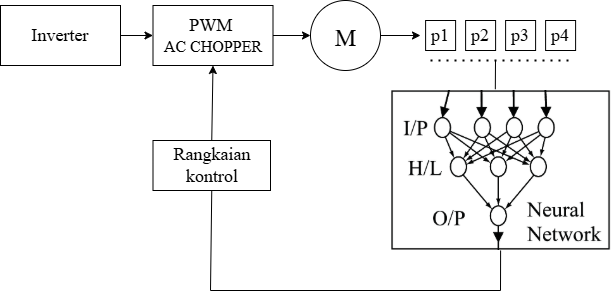
\includegraphics[scale=0.55]{gambar/pwm_ac_rev.drawio.png}
  \caption{Skema Sistem Kontrol PWM AC \emph{Chopper}}
  \label{fig:skema-sistem-kontrol}
\end{figure}

Pada sisi input kontrol, parameter yang dimasukkan ke dalam
\emph{input layer} jaringan saraf adalah \emph{setpoint} tekanan dan
tekanan aktual hasil pembacaan sensor. Keluaran dari jaringan adalah
\emph{duty ratio} PWM yang diterapkan ke \emph{compare register}
(\emph{CCR}) pada \emph{timer} STM32. Dengan pembaruan nilai
\emph{CCR} secara periodik, sistem dapat menyesuaikan tegangan
keluaran PWM AC \emph{chopper} untuk mempertahankan tekanan air
sesuai \emph{setpoint} meskipun terjadi perubahan beban (misalnya
pembukaan atau penutupan keran).

Sensor tekanan yang digunakan adalah DFRobot Analog Water Pressure
Sensor dengan rentang pengukuran 0--1,6 MPa (sekitar 0--16 bar) dan
keluaran analog 0,5--4,5 V. Karena tegangan keluaran sensor tersebut
lebih besar dari tegangan referensi ADC STM32 (3,3 V), digunakan
rangkaian pembagi tegangan untuk membatasi tegangan masuk ke pin
ADC. Persamaan kalibrasi sensor yang digunakan pada penelitian ini
adalah sebagai berikut.

\begin{equation}
  P = a \cdot V_{sensor} + b
  \label{eq:kalibrasi-sensor}
\end{equation}

dengan $P$ adalah tekanan terukur (bar), $V_{sensor}$ adalah tegangan
keluaran sensor setelah melalui pembagi tegangan (V), serta $a$
dan $b$ adalah konstanta kalibrasi yang diperoleh dari regresi linier
antara tegangan sensor dan tekanan referensi. Konstanta $a$ dan $b$
ditentukan dengan membandingkan pembacaan sensor terhadap alat ukur
tekanan referensi pada beberapa titik ukur statis.

\section{Simulasi Rangkaian PWM AC \emph{Chopper} (PSIM)}
\label{sec:simulasi-psim}

Sesuai dengan batasan masalah pada Bab~1, simulasi
rangkaian dilakukan menggunakan perangkat lunak PSIM. Simulasi bertujuan
untuk memvalidasi desain rangkaian daya, menguji keefektifan
\emph{snubber}, dan mengamati karakteristik bentuk gelombang tegangan
keluaran terhadap variasi \emph{duty cycle} dan perubahan beban dinamis
sebelum implementasi pada perangkat keras.

\subsection{Model PSIM dan Skenario Simulasi}
\label{sec:model-psim-dan-skenario}

Model PSIM yang dibangun terdiri atas sumber tegangan AC 220 V/50 Hz
sebagai masukan, rangkaian \emph{full-bridge} empat IGBT sebagai
\emph{chopper}, blok \emph{gate signal} yang menghasilkan sepasang
sinyal PWM komplementer dengan \emph{dead time}, serta blok beban
motor pompa yang dimodelkan sebagai impedansi R-L yang dipasang seri
dengan sumber tegangan \emph{back-EMF} untuk menyederhanakan perilaku
motor AC. Skematik model PSIM ditunjukkan pada
Gambar~\ref{fig:model-psim}.

\begin{figure} [H] \centering
  % Nama dari file gambar yang diinputkan
  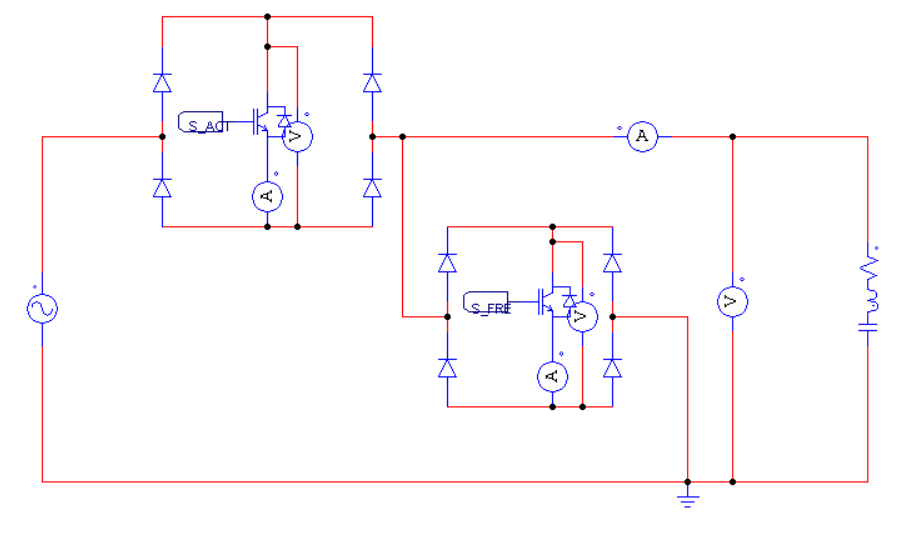
\includegraphics[scale=0.65]{gambar/rangkaian_power.png}
  \caption{Rangkaian Power Simulasi PSIM PWM AC \emph{Chopper}}
  \label{fig:model-psim}
\end{figure}

\begin{figure} [H] \centering
  % Nama dari file gambar yang diinputkan
  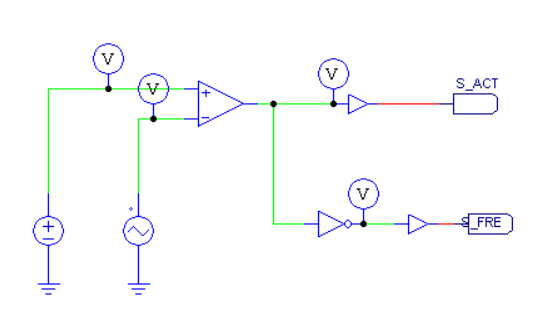
\includegraphics[scale=0.75]{gambar/rangkaian_pwm.png}
  \caption{Rangkaian Sinyal PWM Simulasi PSIM}
  \label{fig:rangkaian-pwm-simulasi}

\end{figure}
Skenario simulasi yang dijalankan adalah sebagai berikut.
\begin{enumerate}
  \item Simulasi variasi \emph{duty cycle} pada 10\%, 20\%, \ldots,
        90\% dengan beban R-L nominal tetap, untuk mendapatkan
        hubungan \emph{duty cycle} terhadap tegangan RMS keluaran dan
        membandingkannya dengan perhitungan teoritis.
  \item Simulasi pengamatan bentuk gelombang tegangan pada sisi
        IGBT ($V_{CE}$) sebelum pemasangan
        \emph{snubber}, untuk memperoleh nilai $V_{spike}$.
  \item Simulasi pengamatan bentuk gelombang yang sama setelah
        pemasangan \emph{snubber} RC, untuk melihat reduksi
        \emph{spike} dan \emph{ringing}.
  \item Simulasi perubahan beban secara mendadak (beban dinamis),
        untuk mengamati perilaku sistem ketika impedansi beban
        berubah-ubah sesuai variasi pembukaan keran.
\end{enumerate}

\subsection{Simulasi Efektivitas \emph{Snubber} dan Beban Dinamis}
\label{sec:simulasi-efektivitas-snubber-dan-beban-dinamis}

Simulasi efektivitas \emph{snubber} dilakukan dengan cara yang
sama seperti skenario poin 2 dan 3 pada sub-bagian sebelumnya,
yaitu membandingkan bentuk gelombang $V_{CE}$ IGBT ketika
\emph{snubber} belum dipasang dan ketika \emph{snubber} sudah
dipasang. Parameter yang diamati adalah amplitudo $V_{spike}$,
amplitudo dan jumlah siklus \emph{ringing}, serta waktu yang
diperlukan hingga gelombang kembali stabil. Nilai kapasitor
\emph{snubber} $C_s$ dan resistor $R_s$ divariasikan pada
beberapa nilai untuk mendapatkan kombinasi yang memberikan
reduksi lonjakan paling baik tanpa menambah rugi daya yang
berlebihan. Bentuk gelombang hasil simulasi sebelum dan sesudah
\emph{snubber} ditunjukkan pada Gambar~\ref{fig:simulasi-snubber}.

\begin{figure} [H] \centering
  % Nama dari file gambar yang diinputkan
  
\includegraphics[scale=0.5]{gambar/simulasi_snubber.png}
  \caption{Perbandingan Bentuk Gelombang IGBT Sebelum dan Sesudah
           \emph{Snubber}}
  \label{fig:simulasi-snubber}
\end{figure}

Simulasi beban dinamis dilakukan dengan memvariasikan nilai
resistansi dan induktansi beban dalam rentang waktu tertentu,
misalnya pada $t = 0{,}5$ s beban berubah dari kondisi
\textit{semua keran tertutup} menjadi \textit{satu keran
terbuka}, dan pada $t = 1$ s berubah menjadi \textit{dua keran
terbuka}. Bentuk gelombang tegangan dan arus pada terminal
keluaran PWM AC \emph{chopper} diamati untuk memastikan
bahwa sistem dapat mempertahankan operasi yang stabil saat
beban berubah secara mendadak. Hasil simulasi ini selanjutnya
dijadikan acuan awal untuk implementasi pada perangkat keras
nyata.

\section{Implementasi Sistem}
\label{sec:implementasi-sistem}

Bagian ini membahas peralatan yang digunakan dan prosedur
perakitan sistem implementasi, mulai dari perangkat keras
sampai dengan instalasi pada sistem pompa air.

\subsection{Peralatan yang Digunakan}
\label{sec:peralatan-yang-digunakan}

Peralatan yang digunakan pada penelitian ini terdiri atas
perangkat keras dan perangkat lunak. Perangkat keras yang
digunakan beserta spesifikasi pentingnya ditunjukkan pada
Tabel~\ref{tab:perangkat-keras}, sedangkan perangkat lunak
ditunjukkan pada Tabel~\ref{tab:perangkat-lunak}.

\begin{table}[H]
  \centering
  \caption{Daftar Perangkat Keras yang Digunakan}
  \label{tab:perangkat-keras}
  \begin{tabularx}{\linewidth}{|c|>{\raggedright\arraybackslash\hsize=0.7\hsize}X|>{\raggedright\arraybackslash\hsize=1.3\hsize}X|}
  \hline
  \textbf{No.} & \textbf{Perangkat Keras} & \textbf{Spesifikasi / Fungsi} \\
  \hline
  1 & Mikrokontroler STM32 \textit{[seri]} &
      Pembangkit PWM komplementer, ADC sensor tekanan,
      \emph{host} \emph{neural network} \\
  \hline
  2 & IGBT \textit{[tipe]} &
      Saklar daya PWM AC \emph{chopper} full-bridge \\
  \hline
  3 & Rangkaian \emph{gate driver} &
      Pengondisi sinyal PWM dari level logika STM32 ke
      level tegangan gerbang IGBT \\
  \hline
  4 & Rangkaian \emph{snubber} RC &
      Peredam \emph{spike} dan \emph{ringing} pada IGBT \\
  \hline
  5 & Sensor tekanan DF Robot Analog Water Pressure &
      Rentang 0--1{,}6 MPa, keluaran 0{,}5--4{,}5 V \\
  \hline
  6 & Pompa air GP125 125 W 1 fasa &
      Beban utama sistem \\
  \hline
  7 & Keran air (5 buah) &
      Variasi beban (jumlah keran terbuka) \\
  \hline
  8 & Baterai 12 V / \emph{power supply} DC &
      Sumber energi sistem \\
  \hline
  9 & Osiloskop &
      Pengamatan bentuk gelombang PWM dan $V_{CE}$ IGBT \\
  \hline
  10 & Multimeter &
      Pengukuran tegangan dan arus DC/AC \\
  \hline
  11 & \emph{Pressure gauge} referensi &
      Pembanding pembacaan tekanan sensor \\
  \hline
  \end{tabularx}
\end{table}

\begin{table}[H]
  \centering
  \caption{Daftar Perangkat Lunak yang Digunakan}
  \label{tab:perangkat-lunak}
  \begin{tabularx}{\linewidth}{|c|>{\raggedright\arraybackslash\hsize=0.6\hsize}X|>{\raggedright\arraybackslash\hsize=1.4\hsize}X|}
  \hline
  \textbf{No.} & \textbf{Perangkat Lunak} & \textbf{Fungsi} \\
  \hline
  1 & PSIM &
      Simulasi rangkaian daya PWM AC \emph{chopper} \\
  \hline
  2 & EasyEDA &
      Desain skematik dan \emph{layout} PCB \\
  \hline
  3 & STM32CubeIDE &
      Pemrograman firmware STM32 \\
  \hline
  4 & Python (NumPy, Scikit-learn/PyTorch/Keras) &
      Pelatihan dan evaluasi \emph{neural network} \\
  \hline
  \end{tabularx}
\end{table}

\subsection{Perakitan Rangkaian}
\label{sec:perakitan-rangkaian}

Perakitan rangkaian dilakukan setelah desain pada
sub-bab~\ref{sec:desain-pwm-ac-chopper} tervalidasi melalui
simulasi. Skema koneksi keseluruhan sistem implementasi ditunjukkan
pada Gambar~\ref{fig:skema-implementasi}, yang menggambarkan
koneksi antara STM32, \emph{gate driver}, IGBT, sensor tekanan,
dan pompa air.

\begin{figure} [H] \centering
  % Nama dari file gambar yang diinputkan
  
\includegraphics[scale=0.5]{gambar/skema_implementasi.png}
  \caption{Skema Koneksi Keseluruhan Sistem Implementasi}
  \label{fig:skema-implementasi}
\end{figure}

Rangkaian daya dan rangkaian kontrol direalisasikan
\textit{[pilih salah satu atau keduanya: pada PCB fabrikasi
berdasarkan desain EasyEDA / pada \emph{protoboard} atau
\emph{perfboard}]}. Pada tahap ini, perhatian utama diberikan
pada hal-hal berikut.
\begin{enumerate}
  \item Panjang jalur \emph{gate} IGBT diminimalkan untuk
        mengurangi induktansi parasitik yang dapat memicu
        osilasi.
  \item \emph{Snubber} RC dipasang sedekat mungkin dengan
        terminal IGBT.
  \item Catu daya untuk STM32 dan \emph{gate driver} dipisahkan
        untuk mencegah \emph{coupling} derau dari sisi daya.
  \item Kabel daya AC dan jalur sensor dipisahkan secara
        fisik untuk mengurangi interferensi elektromagnetik
        terhadap sinyal ADC.
\end{enumerate}

Setelah perakitan selesai, firmware STM32 di-\emph{flash} melalui
\emph{ST-Link}. Firmware tersebut berisi konfigurasi \emph{timer}
untuk menghasilkan PWM komplementer dengan \emph{dead time},
rutinitas pembacaan ADC untuk sensor tekanan, serta modul
\emph{inference} \emph{neural network} yang akan dibahas pada
sub-bagian~\ref{sec:pelatihan-model-dan-deployment}.

\section{Perancangan \emph{Neural Network}}
\label{sec:perancangan-neural-network}

\emph{Neural network} pada penelitian ini digunakan sebagai
pengendali utama yang memetakan hubungan antara kondisi tekanan
air dan \emph{duty cycle} PWM yang sesuai. Tidak seperti
pengendali konvensional yang memerlukan model matematis plant
secara eksplisit, \emph{neural network} mempelajari pemetaan
\emph{input}--\emph{output} tersebut langsung dari data hasil
eksperimen, sehingga mampu mengikuti karakteristik nonlinier
pompa dan variasi beban keran.

\subsection{Arsitektur dan Parameter}
\label{sec:arsitektur-dan-parameter}

Arsitektur \emph{neural network} yang digunakan adalah
\emph{Multi-Layer Perceptron} (MLP) dengan satu \emph{hidden
layer} (atau dua \emph{hidden layer} jika akurasi belum
mencukupi) yang ditunjukkan pada Gambar~\ref{fig:arsitektur-nn}.

\begin{figure} [H] \centering
  % Nama dari file gambar yang diinputkan
  
\includegraphics[scale=0.5]{gambar/arsitektur_nn.png}
  \caption{Arsitektur \emph{Neural Network} Pengendali
           \emph{Duty Cycle}}
  \label{fig:arsitektur-nn}
\end{figure}

Komposisi \emph{input} dan \emph{output} jaringan adalah
sebagai berikut.
\begin{itemize}
  \item \emph{Input layer}: \emph{setpoint} tekanan
        ($P_{sp}$, bar) dan tekanan aktual
        ($P_{act}$, bar). Opsional dapat ditambahkan
        \emph{error} sebelumnya dan turunannya untuk
        memberikan sifat dinamik pada jaringan.
  \item \emph{Hidden layer}: \textit{[isi jumlah neuron,
        misal 8--16 neuron]} dengan fungsi aktivasi
        \textit{[ReLU / \emph{tanh}]}.
  \item \emph{Output layer}: satu neuron dengan aktivasi
        \emph{sigmoid} yang dinormalisasi ke rentang
        \emph{duty cycle} 0--100\%.
\end{itemize}

Parameter pelatihan yang digunakan pada penelitian ini
ditunjukkan pada Tabel~\ref{tab:parameter-pelatihan-nn}.
Nilai-nilai pada tabel ini akan diisi pada
bab~\ref{chap:hasil_dan_pembahasan} berdasarkan hasil
eksperimen pelatihan.

\begin{table}[H]
  \centering
  \caption{Parameter Pelatihan Model \emph{Neural Network}}
  \label{tab:parameter-pelatihan-nn-desain}
  \begin{tabularx}{\linewidth}{|c|>{\raggedright\arraybackslash\hsize=1.3\hsize}X|>{\centering\arraybackslash\hsize=0.7\hsize}X|}
  \hline
  \textbf{No.} & \textbf{Parameter} & \textbf{Nilai} \\
  \hline
  1 & Jumlah \emph{input} & 2 \\
  \hline
  2 & Jumlah \emph{hidden layer} &  \\
  \hline
  3 & Jumlah neuron tiap \emph{hidden layer} &  \\
  \hline
  4 & Fungsi aktivasi &  \\
  \hline
  5 & Jumlah \emph{output} & 1 \\
  \hline
  6 & Algoritma pelatihan &  \\
  \hline
  7 & \emph{Loss function} &  \\
  \hline
  8 & Jumlah \emph{epoch} &  \\
  \hline
  9 & \emph{Learning rate} &  \\
  \hline
  \end{tabularx}
\end{table}

Alasan pemilihan arsitektur MLP dengan jumlah neuron
yang relatif kecil adalah untuk menjaga agar model
dapat dijalankan pada STM32 yang memiliki memori dan
kapasitas komputasi terbatas. Setiap \emph{forward pass}
di STM32 hanya membutuhkan operasi perkalian--penjumlahan
sederhana dan satu fungsi aktivasi, sehingga waktu
\emph{inference} dapat dipertahankan pada orde milidetik
yang sesuai dengan laju pengambilan data sensor.

\subsection{Akuisisi Dataset dan Pra-Pengolahan}
\label{sec:akuisisi-dataset-dan-pra-pengolahan}

Dataset untuk pelatihan \emph{neural network} diperoleh
dari hasil pengukuran sistem secara langsung. Setiap kali
beban berubah, sistem mencatat nilai \emph{setpoint},
tekanan aktual hasil pembacaan sensor, dan \emph{duty
cycle} yang sedang diberikan. Skenario akuisisi data
meliputi pembukaan keran secara bertahap, mulai dari
semua keran tertutup, satu keran terbuka sebagian, satu
keran terbuka penuh, dua keran terbuka, sampai lima
keran terbuka. Format dataset hasil akuisisi ditunjukkan
pada Tabel~\ref{tab:format-dataset-akuisisi}, dan
contoh template dataset untuk pelatihan ditunjukkan pada
Tabel~\ref{tab:dataset-template}.

\begin{table}[H]
  \centering
  \caption{Format Dataset Hasil Akuisisi Data}
  \label{tab:format-dataset-akuisisi-desain}
  \begin{tabularx}{\linewidth}{|c|>{\raggedright\arraybackslash\hsize=0.9\hsize}X|>{\raggedright\arraybackslash\hsize=1.3\hsize}X|>{\centering\arraybackslash\hsize=0.8\hsize}X|}
  \hline
  \textbf{No.} &
  \textbf{Nama Data} &
  \textbf{Keterangan} &
  \textbf{Satuan} \\
  \hline
  1 & Waktu pengambilan data &
      Waktu data diterima oleh komputer & detik \\
  \hline
  2 & ADC sensor tekanan &
      Nilai digital hasil pembacaan ADC STM32 & bit \\
  \hline
  3 & Tegangan sensor &
      Tegangan keluaran sensor setelah pembagi tegangan & V \\
  \hline
  4 & Tekanan aktual &
      Tekanan air hasil pembacaan sensor & bar \\
  \hline
  5 & \emph{Duty cycle} &
      Nilai kendali PWM yang diberikan ke rangkaian & \% \\
  \hline
  6 & Frekuensi PWM &
      Frekuensi sinyal PWM dari STM32 & Hz \\
  \hline
  7 & Tegangan RMS keluaran &
      Tegangan keluaran PWM AC \emph{chopper} & V \\
  \hline
  8 & Kondisi beban &
      Kondisi bukaan keran saat data diambil & - \\
  \hline
  \end{tabularx}
\end{table}

\begin{table}[H]
  \centering
  \caption{Tabel Pengambilan Dataset Pengendalian Tekanan
           dengan \emph{Neural Network}}
  \label{tab:dataset-template}
  \begin{tabularx}{\linewidth}{|>{\centering\arraybackslash}X|>{\centering\arraybackslash}X|>{\centering\arraybackslash}X|}
  \hline
  \rowcolor{cyan!20}
  \textbf{Tekanan (Bar)} & \textbf{PWM \emph{Duty Cycle} (\%)} &
  \textbf{Tegangan Output (V)} \\
  \hline
                       &                                  &                            \\
  \hline
                       &                                  &                            \\
  \hline
                       &                                  &                            \\
  \hline
                       &                                  &                            \\
  \hline
                       &                                  &                            \\
  \hline
                       &                                  &                            \\
  \hline
                       &                                  &                            \\
  \hline
  \end{tabularx}
\end{table}

Sebelum digunakan untuk pelatihan, seluruh fitur input
dinormalisasi ke rentang $[0, 1]$ menggunakan
\emph{min-max normalization} dengan persamaan berikut.

\begin{equation}
  x_{norm} = \frac{x - x_{min}}{x_{max} - x_{min}}
  \label{eq:normalisasi}
\end{equation}

dengan $x$ adalah nilai fitur asli, $x_{min}$ dan
$x_{max}$ adalah nilai minimum dan maksimum fitur
tersebut pada dataset. Normalisasi dilakukan agar
proses pelatihan tidak didominasi oleh fitur dengan
rentang nilai yang besar dan agar \emph{forward pass}
pada STM32 dapat dilakukan dengan aritmatika titik
tetap (\emph{fixed-point}) tanpa overflow. Dataset
selanjutnya dibagi menjadi data latih, data validasi,
dan data uji dengan proporsi seperti pada
Tabel~\ref{tab:pembagian-dataset-desain}. Nilai proporsi
diambil sebagai acuan awal dan akan dilaporkan secara
kongkrit pada
bab~\ref{chap:hasil_dan_pembahasan}.

\begin{table}[H]
  \centering
  \caption{Pembagian Dataset \emph{Neural Network}}
  \label{tab:pembagian-dataset-desain}
  \begin{tabularx}{\linewidth}{|c|>{\raggedright\arraybackslash}X|>{\centering\arraybackslash}X|>{\centering\arraybackslash}X|}
  \hline
  \textbf{No.} & \textbf{Jenis Data} & \textbf{Persentase} &
  \textbf{Jumlah Data} \\
  \hline
  1 & Data latih & 70\% &  \\
  \hline
  2 & Data validasi & 15\% &  \\
  \hline
  3 & Data uji & 15\% &  \\
  \hline
  \end{tabularx}
\end{table}

\subsection{Pelatihan Model dan \emph{Deployment} ke STM32}
\label{sec:pelatihan-model-dan-deployment}

Pelatihan model \emph{neural network} dilakukan di PC
menggunakan bahasa pemrograman Python dan pustaka
\textit{[isi pustaka yang dipakai]} dengan parameter
yang tercantum pada
Tabel~\ref{tab:parameter-pelatihan-nn-desain}. Proses
pelatihan dijalankan hingga \emph{loss} pada data
validasi tidak lagi menurun secara signifikan, dan
model dengan kinerja terbaik pada data validasi
disimpan untuk tahap \emph{deployment}.

Setelah model terbaik diperoleh, bobot dan bias pada
setiap layer diekstrak ke dalam bentuk \emph{array}
\texttt{float} (atau dikuantisasi ke \texttt{int16}
jika diperlukan). Konstanta normalisasi $x_{min}$,
$x_{max}$, $y_{min}$, dan $y_{max}$ juga diekstrak
untuk digunakan pada tahap denormalisasi di STM32.
Seluruh nilai tersebut kemudian disalin ke dalam
\emph{array} \texttt{const} pada firmware STM32,
sehingga menjadi bagian dari \emph{image} program
yang akan di-\emph{flash} ke mikrokontroler.

Pada STM32, modul \emph{inference} dijalankan pada
setiap periode sampling kendali dengan urutan sebagai
berikut.
\begin{enumerate}
  \item Membaca nilai ADC sensor tekanan dan mengonversinya
        menjadi tekanan aktual $P_{act}$ menggunakan
        Persamaan~\ref{eq:kalibrasi-sensor}.
  \item Menyusun \emph{vector input}
        $\mathbf{x} = [P_{sp}, P_{act}]^T$ dan
        menormalisasikannya menggunakan
        Persamaan~\ref{eq:normalisasi}.
  \item Melakukan \emph{forward pass} MLP
        (perkalian matriks--vektor dan penerapan fungsi
        aktivasi) untuk mendapatkan output ternormalisasi
        $\hat{y}_{norm}$.
  \item Mendelormalisasi $\hat{y}_{norm}$ kembali ke
        rentang \emph{duty cycle} 0--100\% dan menuliskan
        nilainya ke \emph{Compare Register} (\emph{CCR})
        \emph{timer} STM32, sehingga \emph{duty cycle}
        PWM yang baru langsung diterapkan pada IGBT.
\end{enumerate}

Dengan alur ini, \emph{neural network} bertindak
sebagai \emph{controller} adaptif yang seluruh proses
\emph{inference}-nya berjalan di dalam STM32 secara
\emph{real-time}, sementara proses pelatihan tetap
dilakukan di PC secara \emph{offline}. Pemisahan ini
memanfaatkan kemampuan PC untuk pelatihan yang intensif
sumber daya, dan menjaga agar STM32 hanya menjalankan
komputasi ringan pada setiap siklus kendali.

\section{Urutan Pelaksanaan dan Jadwal Penelitian}
\label{sec:urutan-dan-jadwal}

\subsection{Diagram Alir Penelitian}
\label{sec:diagram-alir-penelitian}

Urutan pelaksanaan penelitian tugas akhir ini mengikuti
diagram alir pada Gambar~\ref{fig:urutan}. Penelitian
dimulai dengan studi literatur, kemudian perancangan
rangkaian PWM AC \emph{chopper} dan sistem kontrol
STM32, lalu simulasi dengan PSIM, implementasi perangkat
keras, akuisisi dataset, pelatihan \emph{neural
network}, \emph{deployment} ke STM32, pengujian
terintegrasi, dan diakhiri dengan analisis hasil serta
penulisan buku tugas akhir. Tempat pelaksanaan
penelitian dilakukan di Laboratorium Mikroelektronika
dan Sistem Tertanam Departemen Teknik Elektro Institut
Teknologi Sepuluh Nopember selama lima bulan.

\begin{figure} [H] \centering
  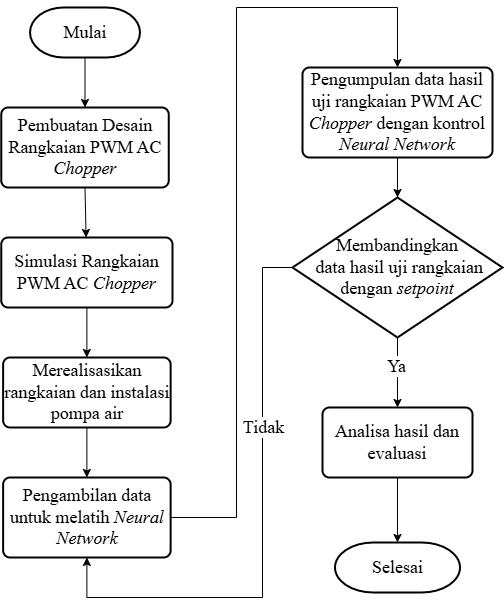
\includegraphics[scale=0.50]{gambar/dalirpenelitian.drawio.png}
  \caption{Diagram alir urutan pelaksanaan tugas akhir}
  \label{fig:urutan}
\end{figure}

\subsection{Jadwal Pelaksanaan}
\label{sec:jadwal-pelaksanaan}

\newcommand{\w}{}
\newcommand{\G}{\cellcolor{blue}}
\begin{table}[H]
  \captionof{table}{Tabel jadwal pelaksanaan tugas akhir}
  \label{tbl:timeline}
  \begin{tabularx}{\linewidth}{|>{\raggedright\arraybackslash}X|c|c|c|c|c|c|c|c|c|c|c|c|c|c|c|c|}

    \hline
    \multirow{2}{*}{Kegiatan} &
    \multicolumn{16}{|c|}{Minggu} \\
    \cline{2-17}              &
    1 & 2 & 3 & 4 & 5 & 6 & 7 & 8 &
    9 & 10 & 11 & 12 & 13 & 14 & 15 & 16 \\
    \hline

    % Gunakan \G untuk mengisi sel dan \w untuk mengosongkan sel
    Studi Literatur          &
    \G & \G & \w & \w & \w & \w & \w & \w &
    \w & \w & \w & \w & \w & \w & \w & \w \\
    \hline

    Desain Rangkaian PWM AC \emph{chopper}           &
    \w & \w & \G & \G & \G & \w & \w & \w &
    \w & \w & \w & \w & \w & \w & \w & \w \\
    \hline

    Simulasi Rangkaian PWM AC \emph{chopper}             &
    \w & \w & \w & \w & \w & \G & \G & \w &
    \w & \w & \w & \w & \w & \w & \w & \w \\
    \hline

    Pembuatan Rangkaian dan Instalasi Sistem Pompa Air      &
    \w & \w & \w & \w & \w & \w & \w & \G &
    \G & \G & \G & \w & \w & \w & \w & \w \\
    \hline

    Akuisisi Dataset dan Pelatihan \emph{Neural Network}       &
    \w & \w & \w & \w & \w & \w & \w & \w &
    \w & \G & \G & \G & \G & \w & \w & \w \\
    \hline

    \emph{Deployment} dan Pengujian Sistem       &
    \w & \w & \w & \w & \w & \w & \w & \w &
    \w & \w & \w & \G & \G & \G & \G & \G \\
    \hline

    Penulisan Buku Tugas Akhir      &
    \w & \w & \w & \w & \w & \w & \w & \w &
    \w & \w & \w & \w & \w & \G & \G & \G \\
    \hline


  \end{tabularx}
\end{table}